\documentclass[aspectratio=169]{beamer}
\setbeamertemplate{navigation symbols}{}
\usepackage{color, amsmath, comment, subfigure}
\usepackage{url}

\usepackage{hyperref}
\hypersetup{
    colorlinks=true,
    linkcolor=blue,
    filecolor=magenta,      
    urlcolor=cyan,
}

%%%%%%%%%%%%%%%%%%%%%%%%%%
\title[]{Pre-read for Thursday, October 8:\\Social fads, part 2}
\author[]{Matthew J. Salganik}
\institute[]{}
\date[]{COS 597E/SOC 555 Limits to prediction\\Fall 2020, Princeton University}

\begin{document}
%%%%%%%%%%%%%%%%%%%%%%%%%%%
\frame{\titlepage}
%%%%%%%%%%%%%%%%%%%%%%%%%%%
\begin{frame}

\begin{center}
  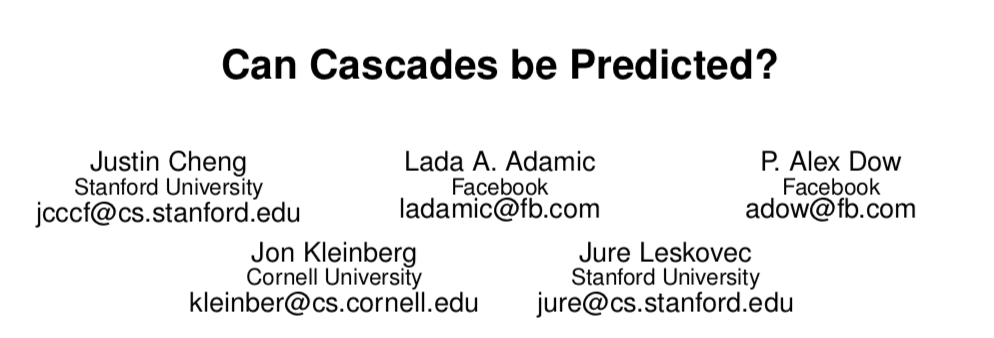
\includegraphics[width = 0.9\textwidth]{figures/cheng_can_2014_title}
\end{center}

\end{frame}
%%%%%%%%%%%%%%%%%%%%%%%%%%%
\begin{frame}

\begin{center}
  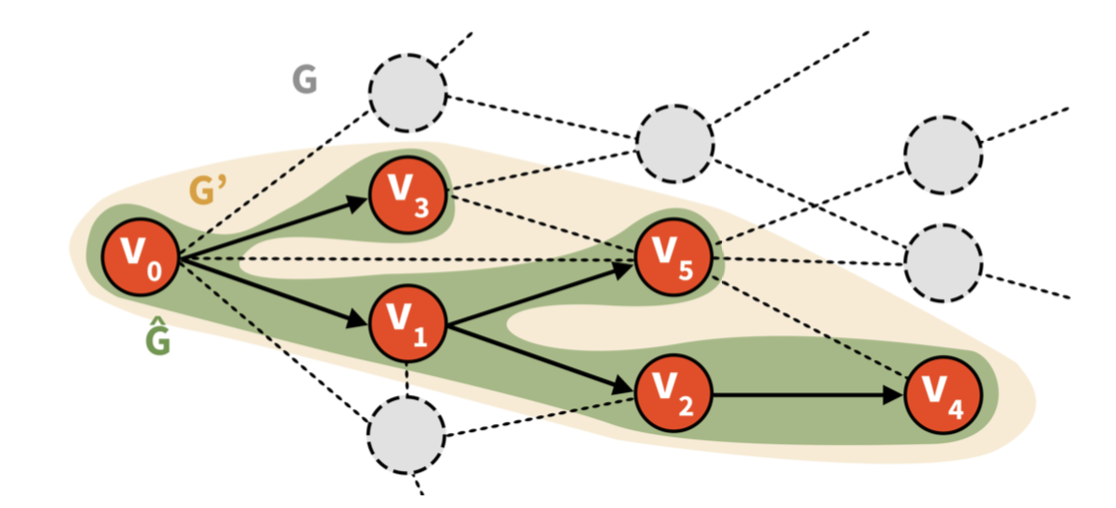
\includegraphics[width = 0.9\textwidth]{figures/cheng_can_2014_fig1}
\end{center}

\end{frame}
%%%%%%%%%%%%%%%%%%%%%%%%%%%%
\begin{frame}

Reading notes:
\begin{itemize}
\item Notice how they formalize the prediction problem.  Martin et al.\ talked about the different between ex ante prediction and ``peeking strategies''.
\pause
\item Facebook might formalize this problem this way because 1) they are looking for viral content to promote and/or 2) they are looking for content that should be prioritized for review.
\pause
\item Note how adding time in this way makes the problem more interesting.
\end{itemize}

\end{frame}
%%%%%%%%%%%%%%%%%%%%%%%%%%%%%
\begin{frame}

\begin{figure}
  
\includegraphics[width = 0.9\textwidth]{figures/goel_predicting_2010_title}
\end{figure}

\end{frame}
%%%%%%%%%%%%%%%%%%%%%%%%%%%%%
\begin{frame}

\begin{figure}
  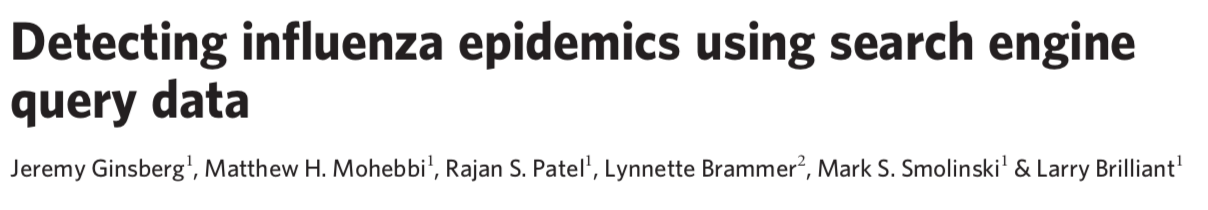
\includegraphics[width = 0.9\textwidth]{figures/ginsburg_detecting_2008_title}
\end{figure}

\end{frame}
%%%%%%%%%%%%%%%%%%%%%%%%%%%%%
\begin{frame}

Reading notes:
\begin{itemize}
\item ``predicting the present'' vs predicting the future
\pause
\item Emphasizes the importance of performance relative to a simple model.  Do you believe this? When might it not be true?
\end{itemize}

\end{frame}
%%%%%%%%%%%%%%%%%%%%%%%%%%%%%
\begin{frame}

One commonality between how these two papers differ from their predecessors: time

\end{frame}
%%%%%%%%%%%%%%%%%%%%%%%%%%%%%




\frame{\titlepage}


\end{document}
